\chapter{Сэдвийн ерөнхий судалгаа}

Сэдвийн хүрээнд өмнө нь ажиллаж үзээгүй олон шинэ технологиудыг судалж, хооронд нь харьцуулан системдээ ашиглахад хамгийн тохиромжтой технологиудыг сонгох, цаашлаад технологийн цар хүрээнд тааруулж системээ хэрхэн өргөжүүлэх боломжтой талаарх мэдлэгийг авлаа. Уг бүлэгт өөрийн хийсэн судалгаан дээрээ үндэслэж сонгосон технологиуд болон веб платформоо бүтээхэд суурь болох ойлголтуудын талаар оруулав.

\section{Үндсэн ойлголтууд}

Уг судалгааны ажлыг амжилттай хийж дуусгахад доорх ойлголтуудыг өөрийн болгосон байх ёстой ба эдгээр үндсэн аргачлалууд дээр манай платформ маань суурилж байгаа билээ.

\subsection{News Aggregation}

Тодорхой ижил контентууд буюу онлайн мэдээ, нийтлэл, подкаст болон видео блогуудыг хялбар байдлаар нэгтгэж харах зориулттай хэрэглэгчид зориулсан веб аппликейшнийг хэлдэг. Өөрөөр хэлбэл олон вебсайтууд дээрх нийтлэлүүдийг хамтад нь нэг хуудаснаас харах, түүнийг унших боломжтой апп юм. Гэхдээ анхаарах зүйл нь өөр вебсайт дээр тавигдсан мэдээллийг бүтнээр нь хуулж авах нь зохиогчийн эрхийн асуудлыг үүсгэдэг. Иймд тухайн мэдээллийн эхний 50 үгийг харуулах эсвэл хэрэглэгчид веб холбоос руу шилжих боломжийг санал болгож өгөх шаардлагатай. News Aggregation нь дотроо хэд хэдэн төрлүүд байдаг ба үүнд 

\begin{itemize}

\item News Aggregator Websites - Өөр өөр төрлийн эх сурвалжуудаас системчлэгдсэн аргаар автоматаар хэрэгтэй мэдээллийг татан авч хэрэглэгчдэд нэгтэн харуулдаг вебсайт
\item Web-Based Feed Readers -  Хэрэглэгчдэд интернэтээс эх сурвалжуудаа олж тухайн үндсэн домайныг өөрийн веб дээрээ нэмэх боломжийг олгосон веб дээр суурилсан систем
\item Feed Reader Applications - Суурин компьютер, гар утас, таблет зэрэг төхөөрөмж дээр суусан мэдээлэл цуглуулах, тэдгээр мэдээллийг бүлэглэн харуулах зориулалттай хэрэглэгч суурьтай интерфейс дизайнтай бүтээгдсэн аппликейшнууд. Хамгийн өргөн хэрэглээтэйд гар утасны имэйл аппууд ордог
\item Social News Aggregators - Интернэт сүлжээнд хамгийн эрэлттэй байгаа мэдээнүүдийг цуглуулж, нэмэлтээр засварлан хүмүүст хүргэх зориулалттай вебсайт эсвэл аппликейшн
\end{itemize}

\subsection{Open Graph Protocol}

Бусад вебсайтууд дээрх мэдээний гарчиг, тайлбар, зураг гэх мэт мэдээллийг авч платформ дээрээ харуулахын тулд Open Graph протоколыг ашиглана. Уг протоколыг 2010 онд Facebook буюу одоогийн Meta компани өөрсдийн сошиал сүлжээндээ ашиглахын тулд гаргаж байсан. Энэхүү протокол нь Facebook сошиал сүлжээндээ бусад вэбсайтуудын тодорхой мэдээллүүдийг хялбараар авч, хэрэглэгчдэд харагдуулах зориулалттай. Open Graph дээр үндсэн 4 tag байдаг ба тус бүр өөрсдийн гэсэн үүрэгтэй. Үүнд

\begin{figure}[h]
	\centering
	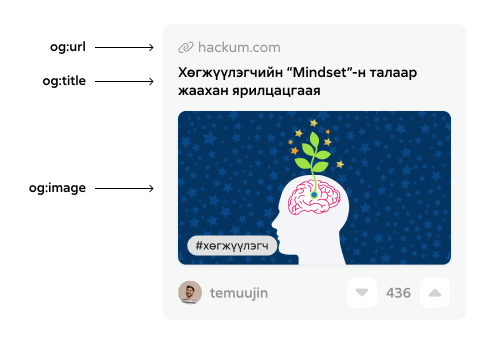
\includegraphics[width=11cm]{images/ogprotocol.png}
	\caption{Open Graph протоколын тагуудын систем дээр ашиглаж буй байдал}
	\label{fig:open-graph-protocol}
\end{figure}

\begin{enumerate}
	\item og:title - Тухайн веб хуудсын гарчиг
	\item og:type - Вебсайтын төрөл
	\item og:image - Тухайн веб хуудас дээрх агуулгыг илэрхийлсэн png, jpg, jpeg форматтай зураг
	\item og:url - Тухайн веб хуудас руу орох холбоос
\end{enumerate} 

Эдгээр tag-ууд нь вебийн HTML хуудасны толгой хэсэгт <meta> tag дотор байрших ба сошиал сүлжээнүүдээс гадна вебийн хандалтыг ихэсгэхийн тулд SEO буюу хайлтын оновчлол дээр ашигладаг. Мөн үндсэн tag-уудаас гадна нэмэлт мэдээллүүдийг агуулсан tag-ууд байдаг.

\section{Ижил төсөөтэй систем}

\subsection{AllTop.com}

AllTop.com вебсайтыг Гая Кавасаки тэргүүтэй гурван залуу нийлж үүсгэн байгуулсан бөгөөд англи хэл дээр бичигдсэн дэлхийн шилдэг эх сурвалжууд руу үсрэх холбоосыг нэгтгэж, төрөлжүүлэн хэрэглэгчдэд харуулдаг News Aggregation төрлийн вебсайт юм. 

\begin{figure}[h]
	\centering
	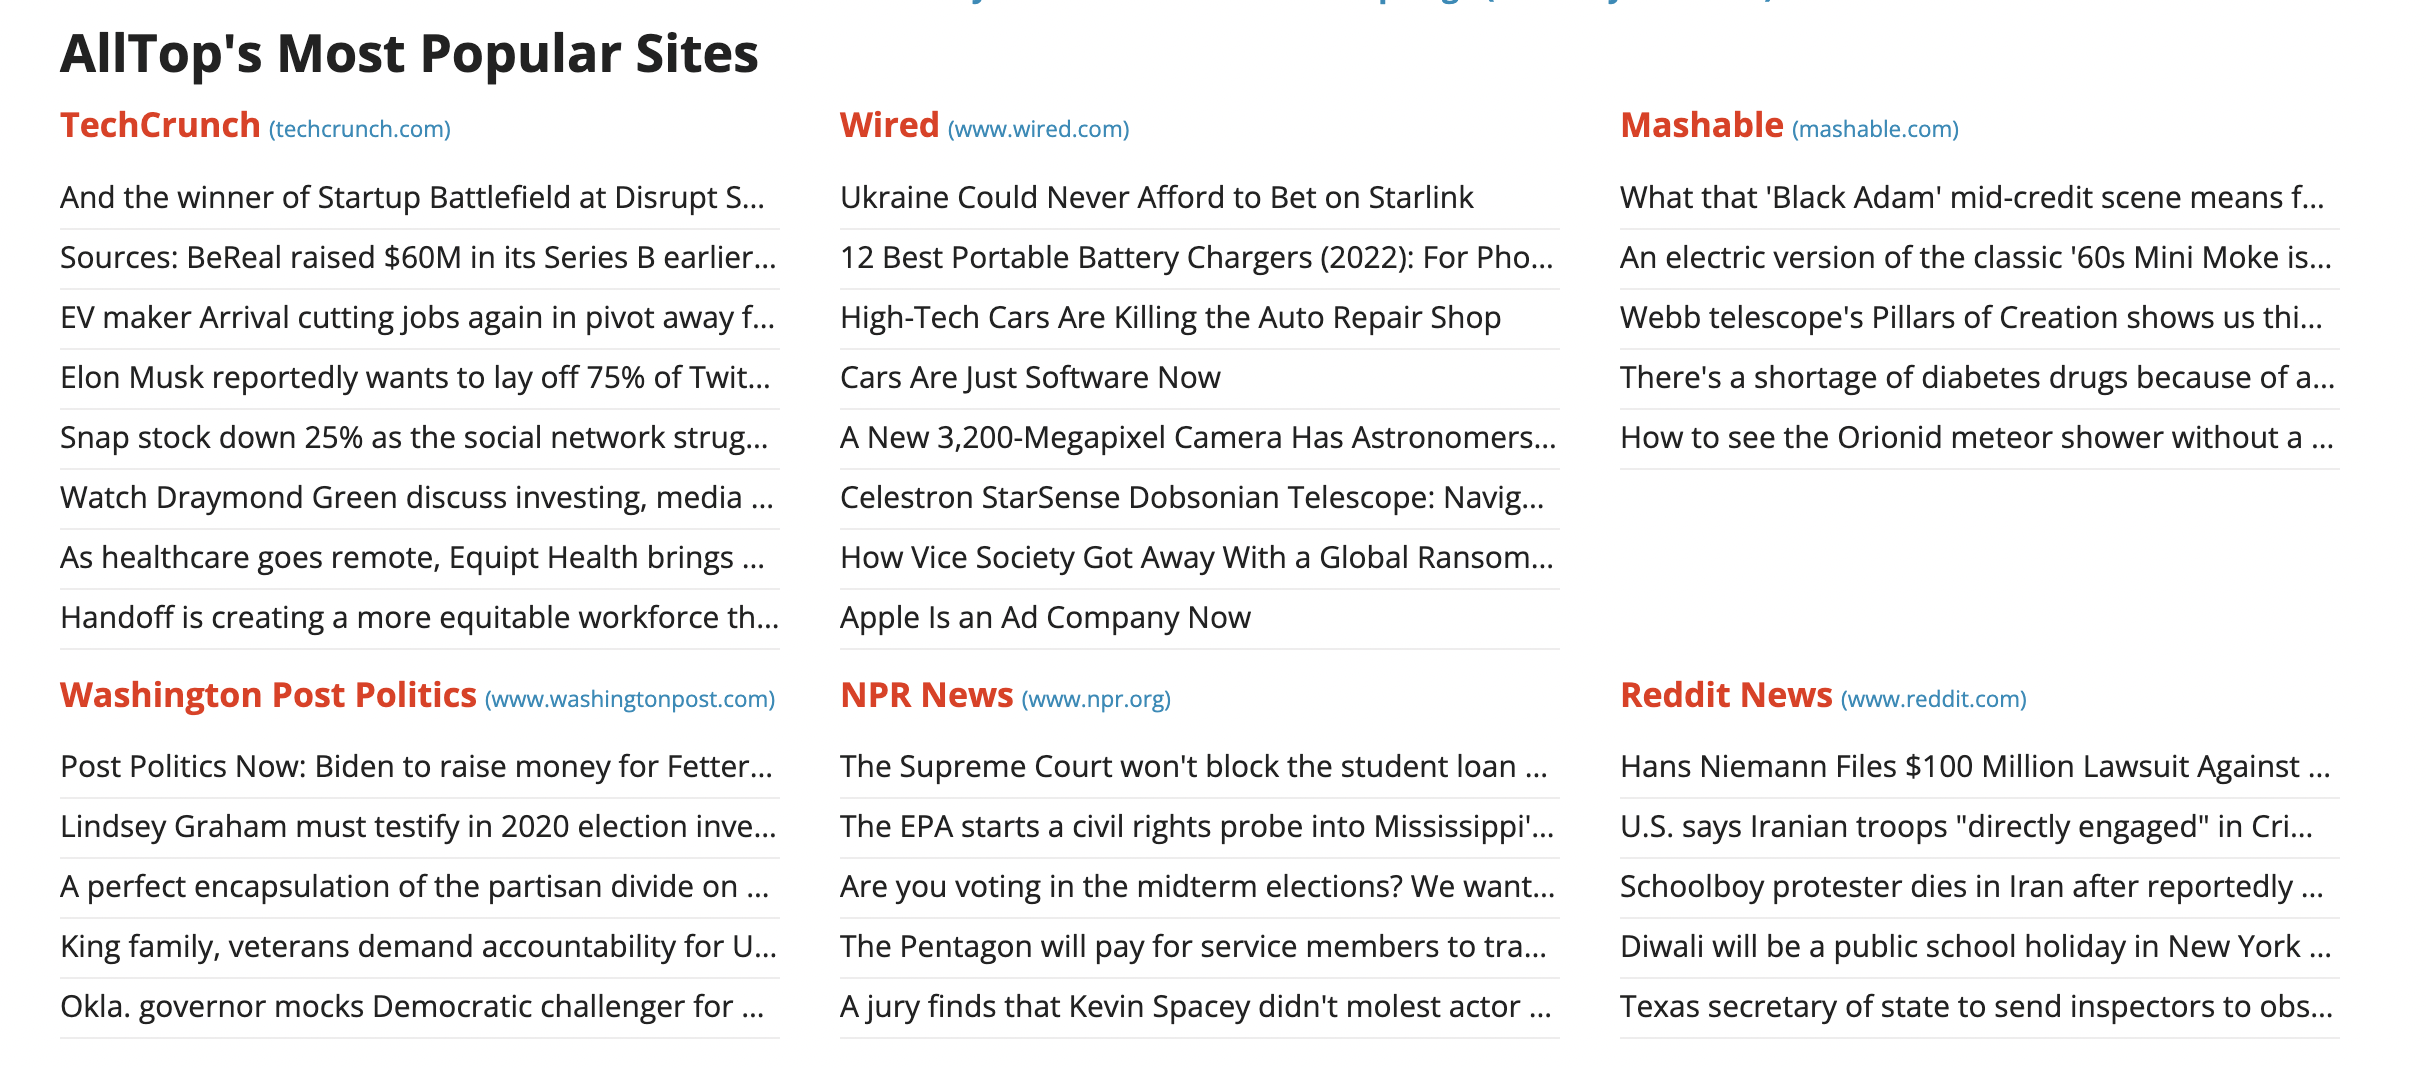
\includegraphics[width=15cm]{images/alltop.png}
	\caption{AllTop.com сайтын харагдах байдал}
	\label{fig:alltop}
\end{figure}

Манай бүтээх гэж байгаа вебээс ялгаатай тал нь 
\begin{itemize}
	\item Зөвхөн RSS feed-тэй сайтууд дээр ажиллах боломжтой
	\item Интерфейсийн хувьд хэт энгийн
	\item Найдвартай эх сурвалжуудаас авна гэсэн учир цаанаасаа тодорхойлж өгсөн хэдэн сайтуудтай
\end{itemize}

Хөгжүүлэлтийн технологийн хувьд Javascript хэл дээр суурилсан jQuery сан болон Bootstrap CSS фрэймворкийг ашиглан бүтээсэн байна. Одоогоор News Aggregation төрлийн вебсайтууд дундаас хамгийн алдартай, хандалт ихтэй сайтуудын нэг бөгөөд үүний гол хүчин зүйл нь энэхүү сайт дээр байх мэдээг бүлэглэж ангилсан байдал болон олон жил тасралтгүй үйл ажиллагаа явуулсан байдал нь илүү хүмүүсийн итгэлийг хүлээсэн гэж үзэж байна. 

\subsection{Linktr.ee}

2016 онд Алекс Закаряа, Антони Закаряа хэмээх ах дүү хоёр дижитал агентийн үйлчилгээ үзүүлдэг компанитай байсан ба захиалагч талдаа зориулж өөрсдийн сошиал хаягуудаа хаяг тус бүрийнхээ bio хэсэгт оруулах шаардлага гарсан байна. Гэвч нэг үйлдлээ олох дахин давтах нь цагийн гарз нэмээд төвөгтэй санагдсан тул өөрсдийн сошиал хаягууд нь нэг дор байрладаг, удирдах боломжтой платформын санаа гаргаж хөгжүүлж эхэлсэн байна. Өдгөө дэлхий даяар нийт 23 сая идэвхтэй хэрэглэгчтэй болж чадсан бөгөөд 2020 онд Reddit-н удаах шилдэг сошиал вебсайтаар шалгаржээ. 

Онцлог нь гэвэл хэрэглэгч тус бүр өөр өөрийн веб хуудас үүсгэх ба түүн дээрээ бүхий л сошиал хаягуудаа сонирхолтой байдлаар жагсааж бусад хүмүүст харуулах боломжтой. Мөн таны хуудсыг нийт хэдэн хүн үзсэн, хэдэн удаа даралт авсан гэх мэт тоо баримтыг танд гаргаж өгч чадна. Интерфейс дизайны хувьд шинэлэг байгаа нь хамгийн том давуу тал гэж үзэж байна. 

\begin{figure}[h]
	\centering
	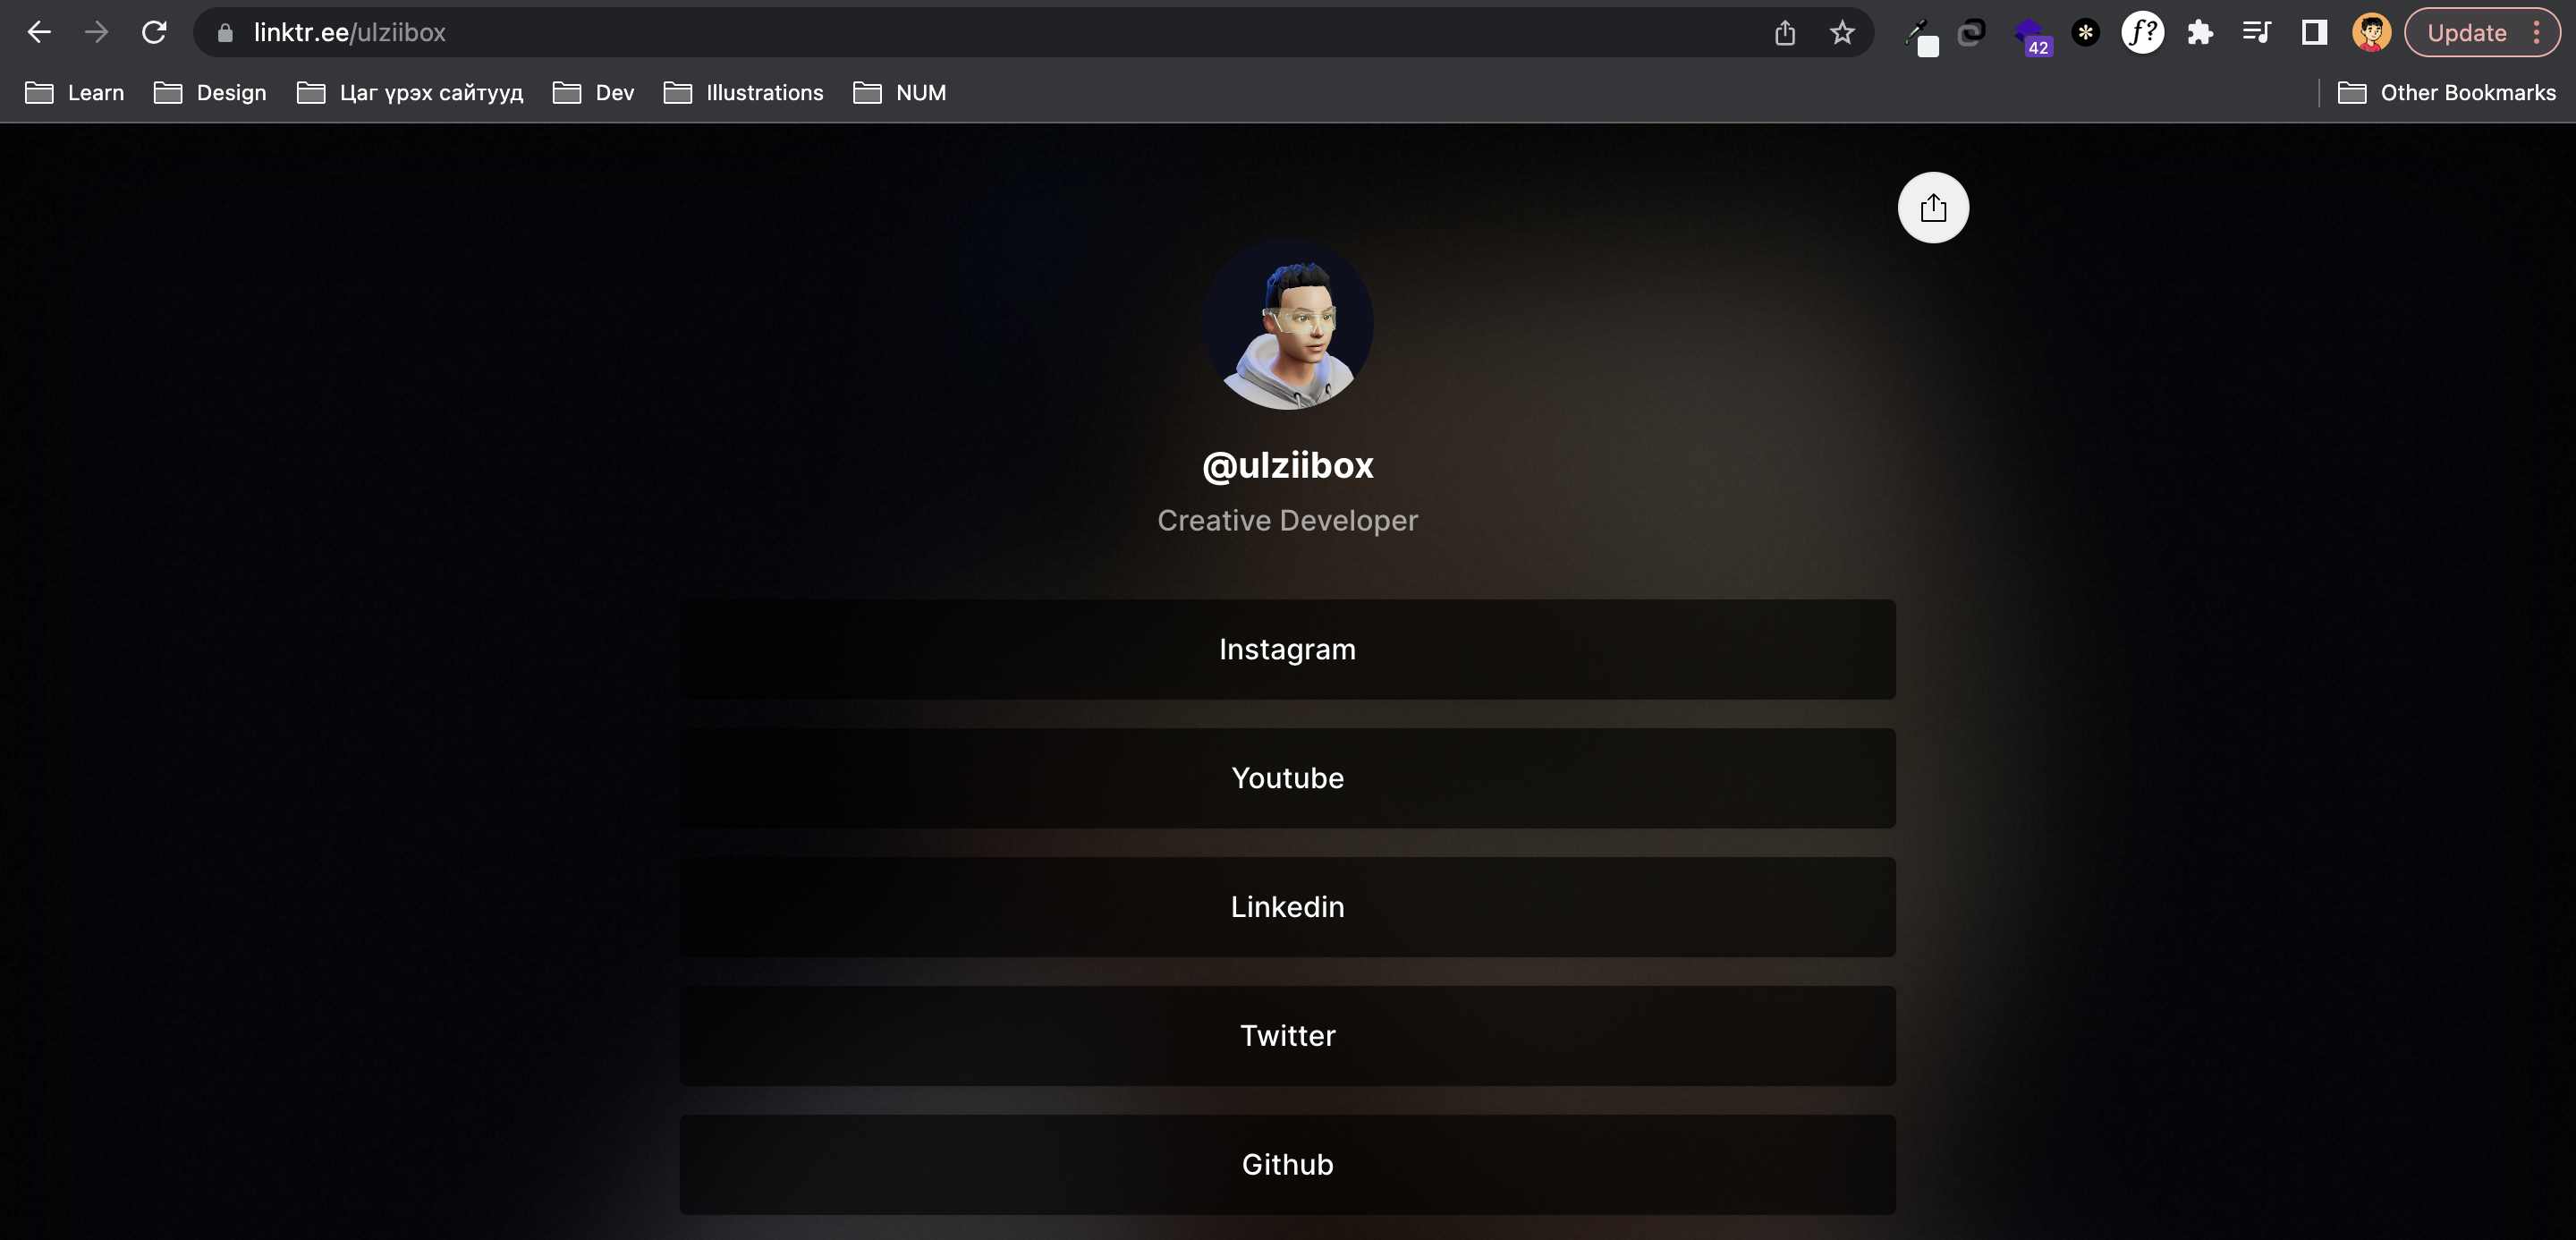
\includegraphics[width=15cm]{images/linktree.png}
	\caption{Linktr.ee сайтын харагдах байдал}
	\label{fig:linktree}
\end{figure}

Уг сайтын хөгжүүлэлтийн технологийн хувьд гэвэл харьцангүй сүүлд гарсан веб учир React дээр суурилсан Next.js фрэймворк болон Node.js ашиглажээ. CSS дээрээ styled-component-г ашигласан нь өөрсдийн онцлог интерфейс дизайнаа бүтээхэд илүү хялбар байсан талаар хөгжүүлэгчид нь дурдсан байна.

\section{Ашиглах технологи}

\subsection{React - Javascript сан}

\subsubsection{Сонгосон шалтгаан}

Хэдийгээр олон төрлийн технологи ашиглан уг бүтээгдэхүүнийг хөгжүүлэх боломжтой ч орчин үед хамгийн трэнд болж буй уг технологийн тусгайлан сонгож аван судалж үзлээ. Хамгийн эхлээд 2022 онд хамгийн ихээр ашиглаж буй вэб фрэймворкийн судалгааг \footnote{Вэб фрэймворкийн судалгаа \url{https://www.statista.com/statistics/1124699/worldwide-developer-survey-most-used-frameworks-web/}} танилцуулъя. 

\begin{figure}[h]
	\centering
	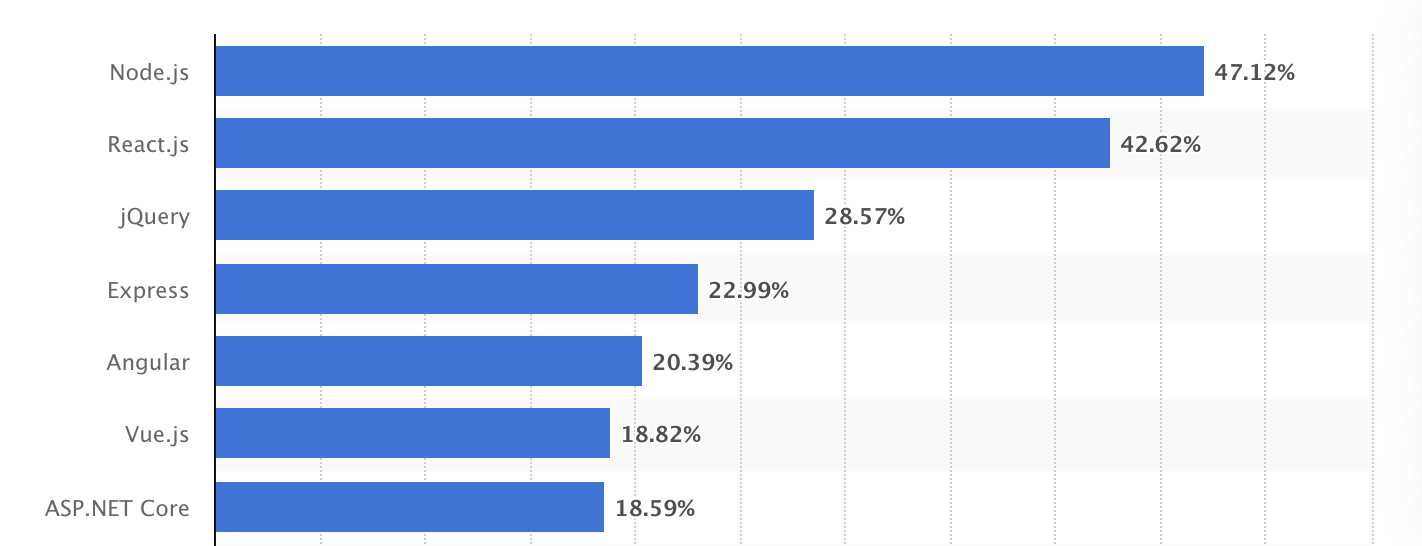
\includegraphics[width=12cm]{images/most-used-frameworks.png}
	\caption{2022 онд хамгийн ихээр ашиглаж буй вэб фрэймворкийн жагсаалт}
	\label{fig:most-used-frameworks}
\end{figure}

Энэ судалгаанаас та React.js-г вэбийн Front-End хэсэг дээр хамгийн ихээр ашиглаж буйг харж болно.

Мөн Javascript хэл ашиглан хийсэн, хөгжүүлэлт хийхэд хялбар, client болон server-side аппликейшн хийх боломжтой, виртуал DOM гэсэн ойлголтыг оруулж ирснээр бусад сангуудаас илүү хурдан ажиллах боломжийг олгосон нь уг санг сонгосон хамгийн том шалтгаанууд юм. 

\subsubsection{Технологийн талаар}

Фэйсбүүк компани дотооддоо ашиглаж байсан технологио 2013 онд танилцуулсан нь програмчлалын Javascript хэлийг ашиглаж хийсэн Front-end library болох React\footnote{Reactjs official site \url{https://reactjs.org}} технологи юм. Declarative UI хөгжүүлэлтийн аргыг хамгийн анх дэлгэрүүлж, өргөн хэрэглээнд нэвтрүүлж чадсан тул Declarative UI-н гол төлөөлөгч гэж явдаг. Уг технологийг ашиглахын тулд үндсэн хэдэн ойлголтууд авах хэрэгтэй. Үүнд component ба түүний lifecycle, javascript-н өргөжүүлсэн хувилбар болох jsx, мөн хамгийн чухал зүйл болох Virtual DOM нар багтана. 

Declarative UI гэдэг нь хэрэглэгчийн интерфейсийн кодыг бичихдээ юу зурагдах буюу render хийх үеийн интерфейсийг бүгдийг урьдчилан тодорхойлдог арга барил юм. Imperative програмчлалаас ялгаатай нь хязгаартай нөхцөлд яг юу хийхийг хатуугаар зааж өгөхгүйгээр тухайн state-с хамааруулж хэрэглэгчийн хүссэн зүйлийг гаргаж өгөх боломжтой.   

React нь component-based буюу DOM дээр хэвлэж байгаа бүх зүйлс component байна гэсэн дүрмийг баримталдаг. Component үүсгэж бичихийн давуу тал нь нэг бичсэн кодоо олон дахин бичигдэхээс зайлсхийж, дахин ашиглах боломжийг олгодог. Тус бур өөрсдийн гэсэн дотоод төлөвтэй мөн гаднаас утга хүлээн авах чадвартай. Үүнийг бид Props гэж нэрлэдэг. Мөн component нь stateless, stateful гэж хоёр хуваагддаг ба stateful component нь өөрийн гэсэн төлөвтэй, түүнийгээ удирддаг, class болон hook ашигласан функцууд байна. React-н давуу тал нь state эсвэл props-н өөрчлөлтийг үргэлж хянаж байдаг тул өөрчлөлт орж ирэхэд бүтэн хуудсыг зурах бус зөвхөн тухайн өөрчлөгдсөн component-г л дахин зурдаг. Ингэснээр энгийн вебүүдээс илүү хурдтай ажилладаг.

\begin{lstlisting}[language=Javascript, caption=JSX ашиглаж 'container' класстай html элемент буцаах компонент, frame=single]
	export function Container = ({children}) => {
		return (
			<div className="container">
				{children}
			</div>
		)
	}
			
\end{lstlisting}

JSX нь Javascript Extended гэсэн үгний товчлол бөгөөд энгийнээр javascript дотор HTML-н тагуудыг бичиж өгөх мөн кодыг илүү богино болгож хүссэн үр дүндээ хүрэх боломжийг олгодог. Үүний цаана Babel гэсэн transcompiler-г ашиглаж дундын хөрвүүлэлтийг хийдэг ба хэдийгээр HTML таг бичиж байгаа харагддаг ч код дунд цэвэр HTML-г огтоос бичиж өгдөггүй гэсэн үг юм \footnote{Дадлагын хугацаандаа хийж байсан технологийн судалгаанаасаа иш татав \url{https://github.com/ulziibox/intern-report/blob/main/main.pdf}}. 


\subsection{Next.js - React дээр суурилсан фрэймворк}

\subsubsection{Сонгосон шалтгаан}

Reactjs өөрийг нь ашиглаж төсөл эхлүүлэхэд router, хуудаслалтаас эхлээд олон төрлийн тохиргоо хийх шаардлагатай болдог нь хөгжүүлэлтийн цагийг их үрдэг. Харин Next.js фрэймворк нь тэр бүх тохиргоог нэг л коммандаар хийж, зөвхөн код дээрээ анхаарал хандуулах боломжийг олгодог нь давуу талтай. Тэгэхээр дан Reactjs дээр төслөө эхлүүлсний оронд фрэймворк ашигласан нь зөв гэж үзлээ.

Next.js давуу талуудаас дурьдвал:
\begin{itemize}
	\item Image Optimization буюу их хэмжээтэй зураг оруулахад автоматаар зургийн чанарыг алдагдалгүйгээр хэмжээг багасгаж өгдөг
	\item Zero config буюу нэг ч тохиргоо хийлгүйгээр төслөө эхлүүлэх боломж
	\item Static Site Generator болон Server Side Render хийх
	\item Typescript болон Fast Refresh дэмждэг
	\item File-system Routing буюу “pages” гэсэн хавтас дотор үүссэн файлуудаас хамаарч вебийн замууд тодорхойлогддог мөн dynamic routing ашиглах боломжтой
	\item API Routes буюу өөр дээрээ nodejs сервер ашиглаж API endpoint гаргах боломжтой. Ингэснээр тусдаа сервер ашиглах шаардлага үүсэхгүй 
	\item SEO буюу хайлтын системийн оновчлолыг SSR ашиглаж тохируулж өгөх гэх мэт маш олон давуу талуудтай
\end{itemize}

Мөн ердөө ганц “build” командаар статик болон динамик вебийг гарган авч ямар нэгэн веб сервер /apache, nginx гэх мэт/ ашиглалгүйгээр сервер дээрээ шууд байршуулах боломжтой юм.

\subsubsection{Технологийн талаар}

Next.js\footnote{Next.js official site \url{https://nextjs.org}} нь React сан дээр суурилж хөгжүүлсэн нээлттэй эхийн фрэймворк бөгөөд Vercel компани 2016 онд албан ёсны танилцуулгаа хийж олон нийтэд зарласан юм. React нь зөвхөн хэрэглэгчийн интерфейсийг зурах үүрэгтэй сан ба бусад веб хөгжүүлэлтэд хэрэгтэй хуудас хооронд шилжих гэх мэт үйлдлийг react-router болон бусад маш олон нэмэлт сангаас сонголт хийж шийдэх шаардлагатай байсан нь төслийн эхлэх явцыг удаашруулах хандлагатай байдаг. Харин Next.js ашигласнаар нэг ч тохиргоо хийлгүйгээр төслийг эхлүүлж шууд код бичих боломжийг бүрдүүлдэг. Цаана нь хийгдсэн тохиргоо нь нийт вебсайтуудын 90 хувийн шаардлагыг хангаж чаддаг гэж үздэг нь уг фрэймворкын сүүлийн жилүүдэд эрэлттэй болж буй шалтгаануудыг нэг билээ.


\subsection{PostgreSQL - Өгөгдлийн сан}

Платформынхоо өгөгдлийн сан дээр ашиглахаар сонгосон PostgreSQL нь 20 жилийн турш идэвхтэйгээр нээлттэй эхээр хөгжүүлэгдэж ирсэн өгөгдлийн сан бөгөөд SQL болон JSON Query дэмждэгээрээ илүү давуу талтай юм. Мөн олон төрлийн ORM дэмжиж ажиллах боломжтой.

Түүхийн хувьд 1986 онд Калифорнийн Их Сургуулийн Компьютерын Ухааны тэнхимд POSTGRES гэдэг нэртэйгээр төсөл нь эхэлжээ. PostgreSQL нь Linux, UNIX (AIX, BSD, HP-UX, SGI IRIX, Mac OS X, Solaris, Tru64) болон Windows үйлдлийн системүүд дээр ажилладгаас гадна Apple, Fujitsu, Red Hat, Cisco, Instagram гэх мэт томоохон компаниуд өөрсдийн зарим бүтээгдэхүүнийхээ технологийн шийдлийг уг өгөгдлийн сан дээр шийдсэн байна.

\subsection{Prisma - Нээлттэй эхийн ORM}

Prisma нь PostgreSQL, MySQL, SQL Server, SQLite болон MongoDB ашиглаж хурдан хугацаанд, алдаа багатай апп бүтээхэд зориулагдаж гарсан нээлттэй эхийн ORM (Object–relational mapping) юм. Нийт 3 хэсгээс бүрдэх ба үүнд 

\begin{enumerate}
	\item Prisma Client - Node.js болон Typescript хэл ашиглаж query бичих багаж
	\item Prisma Migrate - Prisma Cli, Prisma Scheme ашиглан migration хийх багаж
	\item Prisma Studio - GUI ашиглан өгөгдлийн сангаа харах, засвар боломжтой багажууд багтана.
\end{enumerate}

\begin{figure}[h]
	\centering
	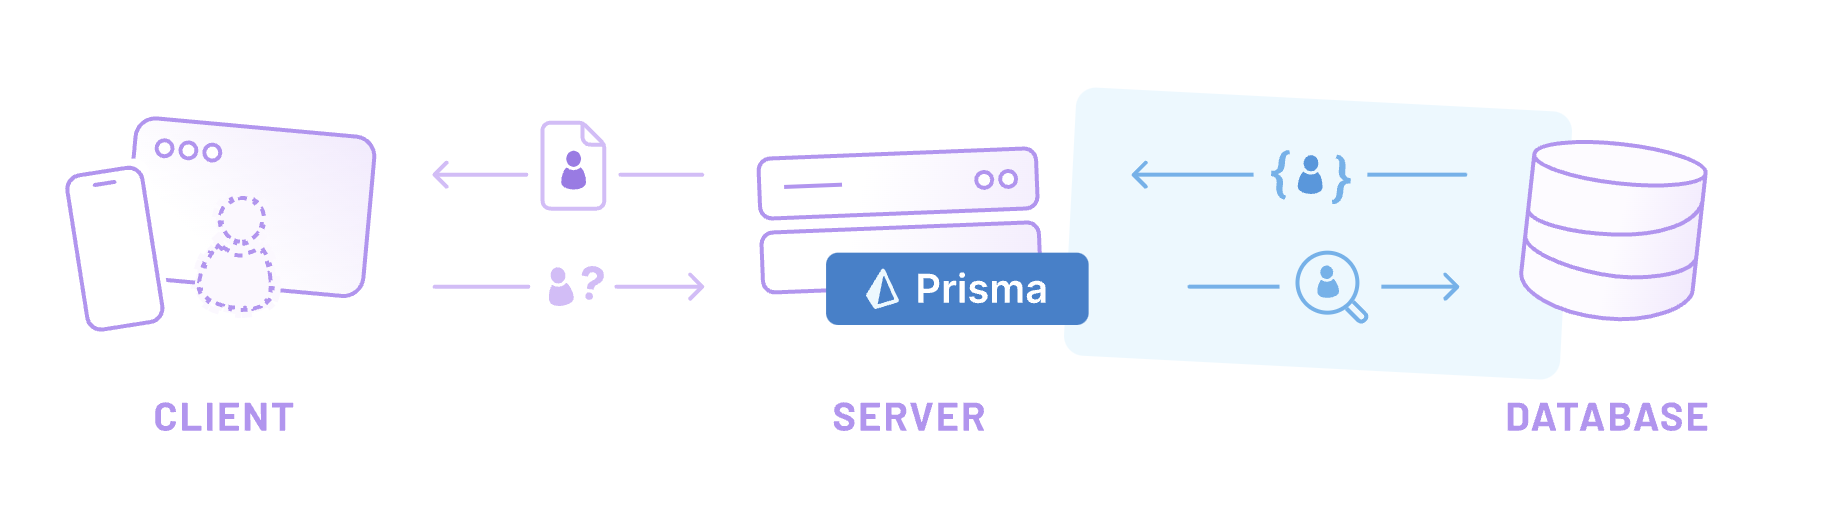
\includegraphics[width=15cm]{images/prisma-stack.png}
	\caption{Prisma тойм зураг}
	\label{fig:prisma}
\end{figure}

Уг технологийг сонгох болсон гол шалтгаан нь Next.js дээр back-end хөгжүүлэлтээ хийхэд Prisma ORM нь хамгийн тохиромжтой гэж үзсэнд ба SQL бичихгүйгээр өгөгдлийн сангаа удирдах боломжтой. Энэ нь миний хувьд илүү хурдан хугацаанд хангалттай үр дүнд хүрэх боломжийг өгч байна.

\subsection{Figma - интерфейс дизайн, Prototype хувилбар гаргах багаж}

Миний хувьд уг платформоо бүтээхдээ хөгжүүлэлтийн үе шатуудыг судлах, түүнийгээ практик дээр хэрэгжүүлэх зорилготой байгаа эхнээс нь бүхий л зүйлсээ чанартайгаар гүйцэтгэхийг оролдож байгаа. Уг үе шатуудад орчин үеийн аргачлалаар хэрэглэгчийн интерфейс дизайн гаргах, түүнийгээ Prototype түвшинд хүргэж туршиж үзэх нь зайлшгүй багтана. Иймд User Experience болон хэрэглэгчийн интерфейсээ гаргахдаа веб дээр суурилсан Figma гэх багажтай танилцан, ашиглаж байна. 

Figma нь 2015 онд анх үүсэж байсан бөгөөд веб суурьтай тул ямар ч үйлдлийн систем дээр ажиллах боломжтой. Мөн Vector болон Raster төрлийн зурагтай харьдаг, олон дизайнерууд бодит хугацаанд хамтдаа ашиглах боломжтой, веб болон гар утасны аппын интерфейс хөгжүүлэлтэй ижил системээр (жишээ нь адилхан component гэх ойлголттой) явдаг нь үүнийг сонгох хамгийн том давуу тал болж өгсөн.


\begin{figure}[h]
	\centering
	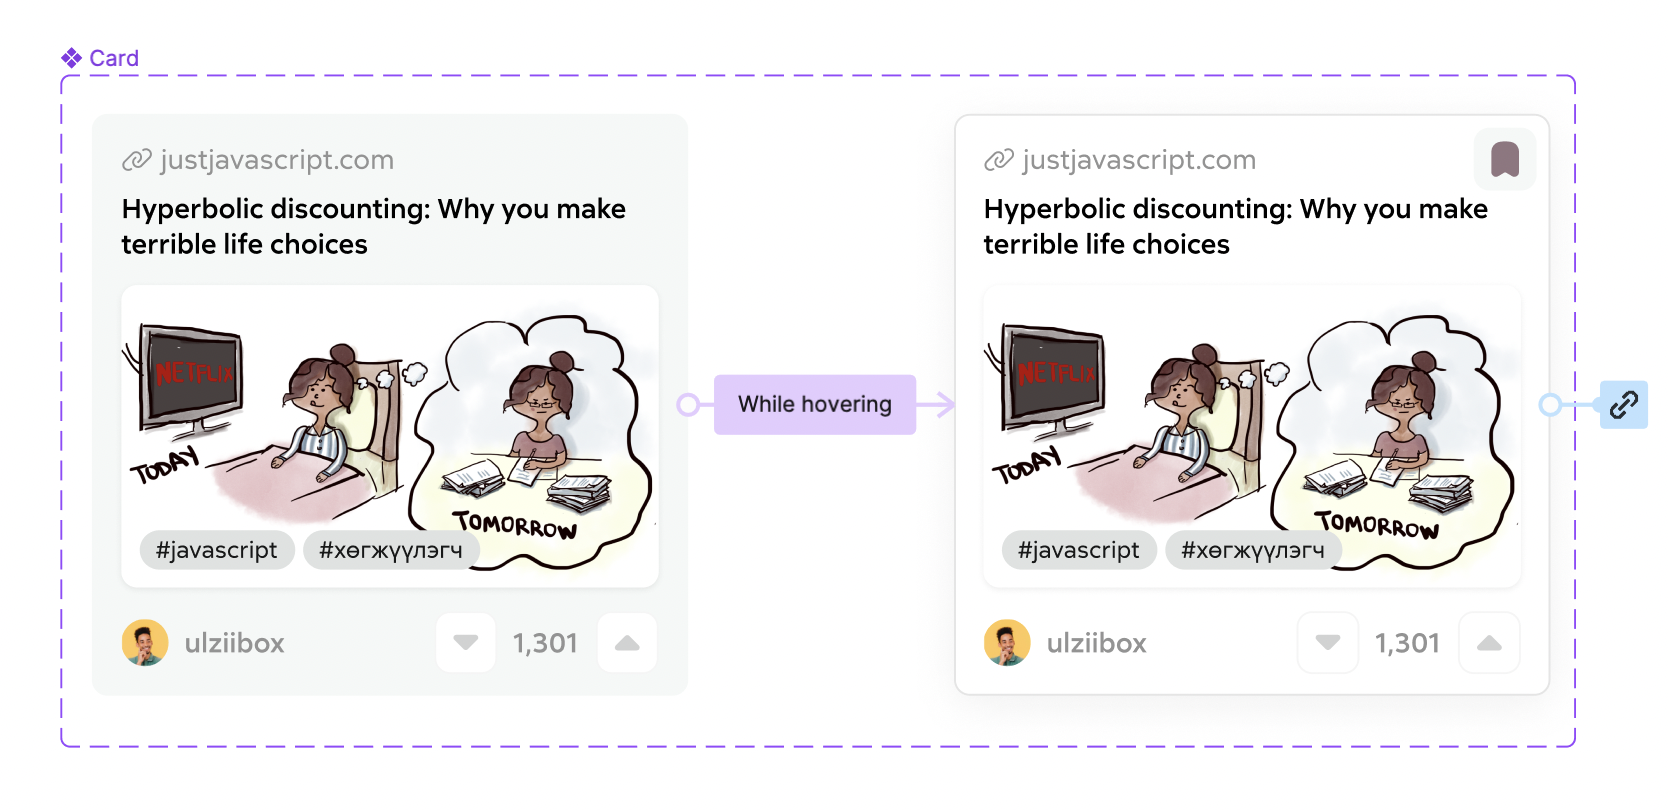
\includegraphics[width=10cm]{images/figma-prototype.png}
	\caption{Figma ашиглаж Card-н hover эффект дээр prototype хийсэн компонент}
	\label{fig:figma}
\end{figure}

Зурсан интерфейсүүдээ хооронд нь холбож хийсвэрээр аппаа ажиллуулан хэрэглэгчийн туршилт хийх хэсгийг Prototype гэдэг бөгөөд заавал кодын хэрэгжүүлэлт хийж цаг хугацаа болон мөнгөн зардал гаргалгүйгээр хийж буй аппаа хэрэглэгчээр туршуулах, үр дүнгээ гарган авч түүнийгээ сайжруулах нөхцөлийг уг веб аппликейшн маань гаргаж өгсөн нь UX/UI дизайнеруудын ашиглах болсон хамгийн том шалтгаануудын нэг юм. 


